\section{Phân tích thiết kế hệ thống}
\label{section4-method}

Như đã trình bày tại phần \ref{section3-background}, hệ thống sẽ bao gồm ba thành phần:
\begin{itemize}
    \item Các thành phần định danh và xác thực: LDAP, Kerberos
    \item Các thành phần lưu trữ và xử lý dữ liệu: HDFS, YARN
    \item Các thành phần quản lý truy cập: Ranger
\end{itemize}

\subsection{Các thành phần định danh và xác thực}

Sử dụng OPENLDAP làm database cho Kerberos, cung cấp định danh để xác thực thông qua ticket. Mô hình xác thực dự kiến như hình \ref{fig:sec4-authen-diagram}

\begin{figure}
    \centering
    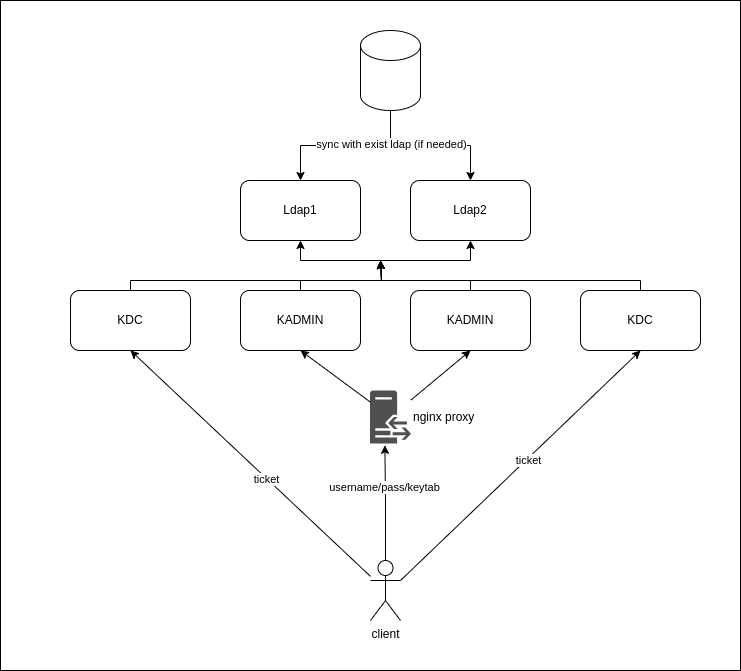
\includegraphics[scale=0.3]{section4/sec4-authen-diagram.png}
    \caption{Sơ đồ tổng quan hệ thống định danh và xác thực}
    \label{fig:sec4-authen-diagram}
\end{figure}

\subsection{HDFS}

Để tăng tính sẵn sàng và chịu lỗi của hệ thống storages, số lượng các node đảm nhiệm các nhiệm vụ khác nhau cần đủ tối thiểu 2, đạt tiêu chuẩn là 3. Mô hình dự kiến như hình \ref{fig:sec4-hdfs-architecture}

\begin{figure}
    \centering
    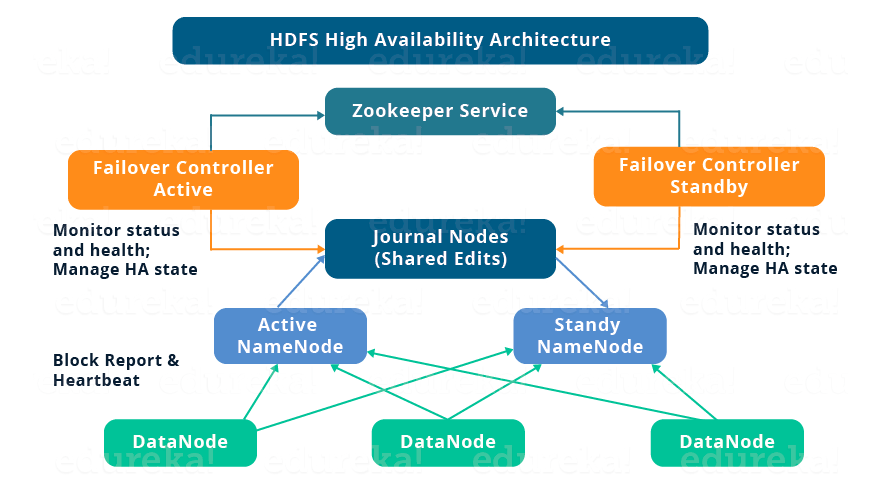
\includegraphics[scale=0.4]{section4/sec4-hdfs-architecture.png}
    \caption{Sơ đồ tổng quan hệ thống hadoop}
    \label{fig:sec4-hdfs-architecture}
\end{figure}

\subsection{Ranger}

Sử dụng Ranger làm admin tool cho config access policy, danh sách user sẽ được sync từ ldap. Các audit log sẽ được lưu lại và hiển thị với từng record. Mô hình dự kiến như hình \ref{fig:sec4-ranger-architecture}

\begin{figure}
    \centering
    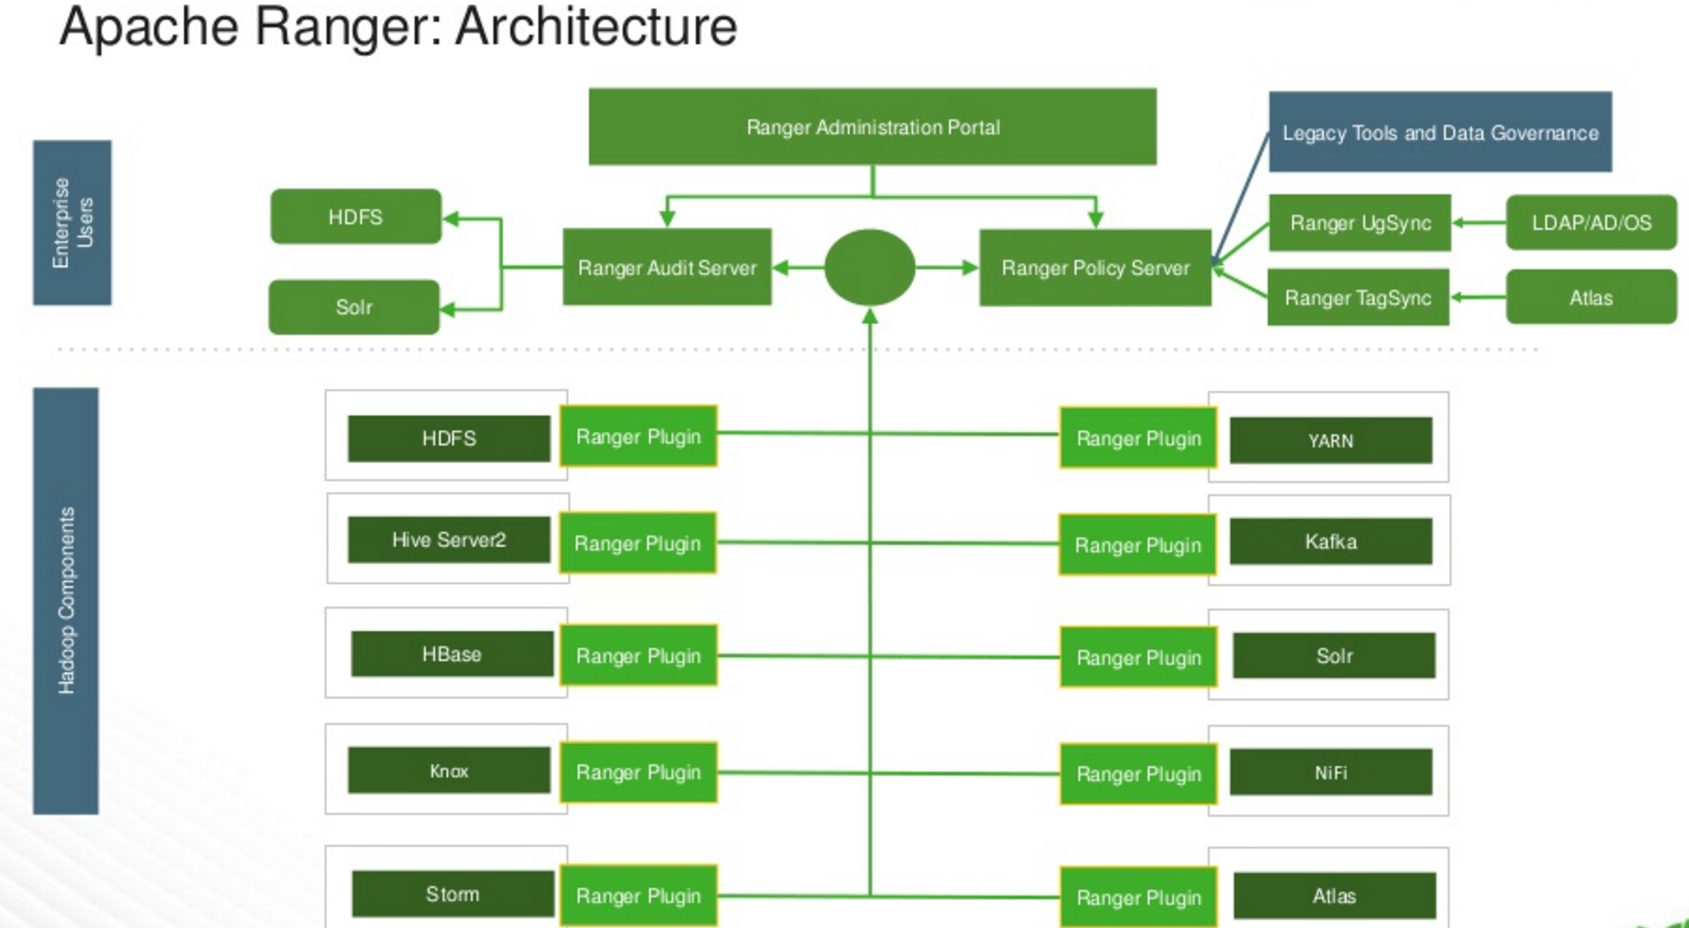
\includegraphics[scale=0.3]{section4/sec4-ranger-architecture.png}
    \caption{Kiến trúc Ranger dự kiến}
    \label{fig:sec4-ranger-architecture}
\end{figure}